\chapter{Introduction}
\label{intro}

Large Reasoning Models (LRMs) represent a breakthrough in AI problem-solving capabilities, yet their effectiveness in interactive environments remains poorly understood. This thesis introduces and analyzes the phenomenon of \textbf{overthinking} in LRMs - a tendency where models prioritize elaborate internal simulations of potential actions over gathering actual environmental feedback. Through extensive experiments on software engineering tasks using SWE Bench Verified, we develop a systematic framework to quantify overthinking behavior on a 0-10 scale, measuring how models balance internal reasoning chains against environmental interaction.

\begin{figure}[t]
    \centering
    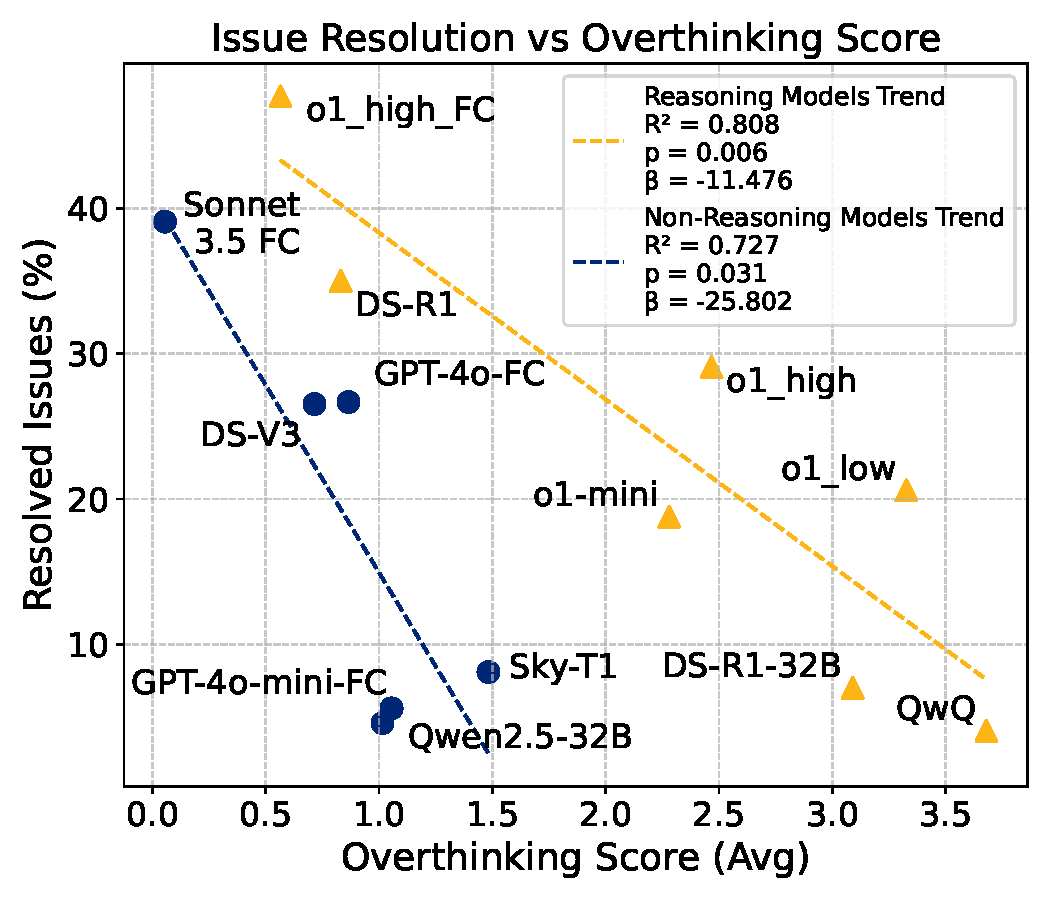
\includegraphics[width=1\linewidth]{model_analysis_combined.pdf}
    \caption{Higher overthinking scores (tendency to favor internal reasoning over environmental feedback) correlate with lower issue resolution rates across all models. Reasoning models exhibit consistently higher overthinking tendencies, suggesting that excessive reliance on internal simulation impairs task performance. Model nomenclature: "FC" indicates native function calling capability, "DS" represents DeepSeek models, and suffixes o1\_high and o1\_low denote models with reasoning effort set to high and low respectively.}
    \label{fig:figure1}
\end{figure}

\begin{figure}[t]
    \centering
    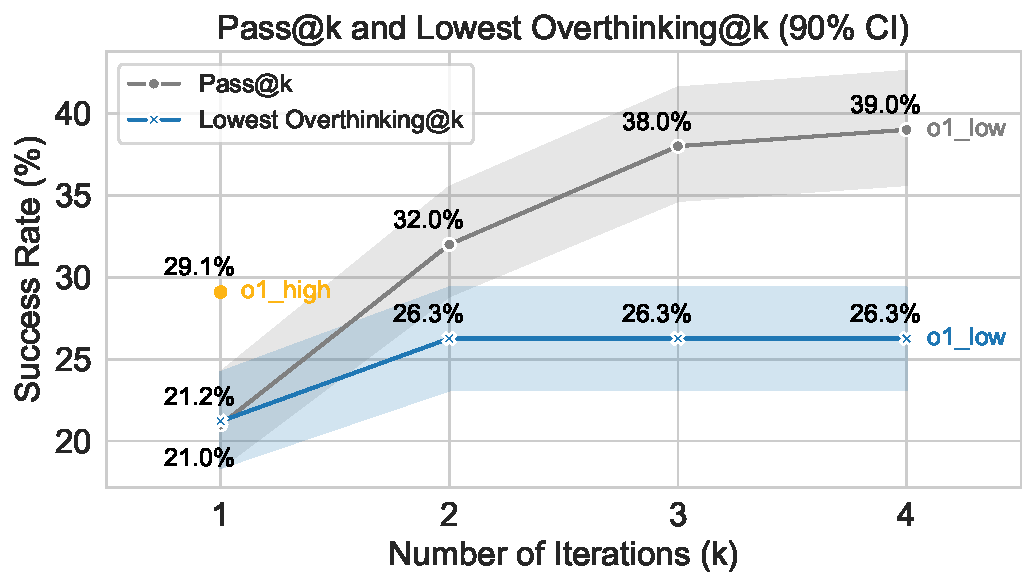
\includegraphics[width=1\linewidth]{pass_at_k_plot.pdf}
    \caption{Pass@k performance for SWE Bench Verified when selecting responses based on overthinking scores. By choosing solutions with minimal overthinking from multiple runs of o1 with low reasoning effort, we achieve performance comparable to high reasoning effort configurations at substantially lower computational cost. The flattening curve suggests diminishing returns from additional iterations, with detailed performance metrics provided in \cref{tab:o1_model_comparison}. The confidence intervals (CI) showcased were computed using Wilson score \cite{wallis2013binomial}.}
    \label{fig:figure2}
\end{figure}

Analysis of \textbf{3,908 trajectories} reveals that overthinking significantly impairs model performance, with strong negative correlations between overthinking scores and issue resolution capabilities (R² = 0.808, p = 0.006 for reasoning models). Notably, LRMs exhibit higher overthinking scores (2.320 ± 1.120) compared to non-reasoning models (0.865 ± 0.432, p = 0.019). Based on our findings, we propose that integrating native function-calling capabilities during training may help models better balance reasoning and action.

\section{The Rise of Large Reasoning Models}
LRMs, defined as LLMs leveraging reinforcement learning techniques for train-time scaling \cite{xu2025largereasoningmodelssurvey}, represent a breakthrough in AI reasoning capabilities \cite{deepseekai2025deepseekr1incentivizingreasoningcapability,openai_o1}. These models are fundamentally built on the principle that allocating more computational resources at test-time enables deeper reasoning \cite{openai_learning_to_reason_2024}. This approach has proven remarkably effective: by dedicating significant compute to deliberate reasoning steps \cite{snell2024scalingllmtesttimecompute}, these models achieve unprecedented performance through extended chain-of-thought reasoning \cite{wei2023chainofthoughtpromptingelicitsreasoning}, systematic exploration of solution strategies, and rigorous self-verification \cite{madaan2023selfrefineiterativerefinementselffeedback}. However, this extended focus on internal reasoning depth raises important questions about how these models balance internal deliberation with action in interactive environments.

\section{The Challenge of Agentic Environments}
While traditional AI defined agents broadly as entities that perceive and act upon their environment \cite{russell1995ai}, the LLM era has evolved toward viewing agency as a spectrum of capabilities \cite{zhang2024agenticinformationretrieval, kapoor2024aiagentsmatter}. Systems are considered more agentic based on three key factors:
\begin{itemize}
    \item Their ability to handle complex environments and pursue goals autonomously
    \item Their capacity to act with minimal supervision through natural language interfaces
    \item Their use of advanced design patterns such as tool utilization and dynamic planning
\end{itemize}

These principles have been extensively applied to software engineering tasks, particularly in solving real-world GitHub issues \cite{jimenez2024swebenchlanguagemodelsresolve}, where numerous research efforts have explored different agent architectures \cite{ibm_swe_agents, aws_q_developer_agent, liu2024marscodeagentainativeautomated, chen2024coderissueresolvingmultiagent, wang2024executablecodeactionselicit} with varying degrees of success. While these efforts have advanced our understanding of AI agents in software engineering, they have not specifically examined how LRMs' unique reasoning capabilities affect their performance in agentic environments—a critical gap our work addresses.

\section{The Reasoning-Action Dilemma}
We observe that, in agentic decision-making tasks, LRMs constantly face the \emph{Reasoning–Action Dilemma} where they must navigate a fundamental trade-off between:
\begin{itemize}
    \item \textbf{Direct interaction with the environment}, where the model executes actions and receives feedback
    \item \textbf{Internal reasoning}, where the model reasons over hypothetical outcomes before committing to an action
\end{itemize}

Ideally, an LRM should balance reasoning and action by using internal simulation to refine its choices while leveraging real-world feedback to correct errors. For instance, when debugging a failing test case, a well-balanced model would hypothesize potential issues yet still execute the test opportunely to collect concrete failure signals.

\section{Contributions}
This thesis makes several key contributions to understanding and addressing the overthinking phenomenon in LRMs:

\begin{enumerate}
    \item We introduce and formalize the concept of overthinking in LRMs, distinguishing it from related phenomena like hallucination
    \item We develop a systematic framework for quantifying overthinking behavior, validated against human expert assessments
    \item We provide extensive empirical evidence of overthinking patterns across different model architectures through analysis of over 3,908 model responses
    \item We demonstrate practical solutions that can improve model performance by 25\% while reducing computational costs by 43\%
\end{enumerate}

\section{Thesis Structure}
The remainder of this thesis is organized as follows:

\begin{itemize}
    \item Chapter \ref{background} provides essential background on LRMs and agentic environments
    \item Chapter \ref{overthinking} introduces our framework for diagnosing and quantifying overthinking
    \item Chapter \ref{evaluation} presents our experimental results and analysis
    \item Chapter \ref{discussion} discusses implications and potential solutions
    \item Chapter \ref{conclusion} summarizes our findings and suggests future research directions
\end{itemize}

To facilitate further research in this direction, we open-source our evaluation framework and comprehensive dataset of annotated model trajectories.
